In this chapter some experiments will be conducted. These experiments are modeled
after the scenarios described in the Theory chapter %TODO ref
The goal is to recreate these situation using the developed tool and running a
simulation with the described parameters. These simulations can then be used
to support or refute the assumptions that were made on how the diseases
theoretically should behave in those scenarios.

\section{Importance of $R_0$}
The role of the reproductive number $R_0$ was discussed in section \ref{sub:r0}.
It is the deciding factor for whether a disease is dying out ($R_0 < 1$) 
or able to live indefinitely ($R_0 > 1$). Calculating $R_0$ in complex social
networks is very hard because the structure of the networks has a big impact on $R_0$
in addition to the characteristics of the disease. For these experiments a very
rough estimation of $R_0=e_\mu \cdot p$ is used as this is sufficient for estimating whether
the disease should die out in the experiment or life for a long time.
$e_\mu$ is the average amount of connection per node, let $N$ be the total
amount of nodes in the network and $E$ the total amount of edges then
$e_\mu=\frac{E}{N}$. $p$ is the probability for a node to get infected
if one of its neighbors has the disease.

\subsection{The network}
\label{sub:exp_network}
The network that is used in these experiments contains 3 groups with 5000 nodes
each. Group 1 has 5 intra group connections for each node, group 2 has 4 and
group 3 has 3 intra group connections. Between each pair of groups there are
2 connections per node. The resulting network can be seen in figure %TODO
It contains a total of 15,000 nodes. Let $N_i$ be the amount of nodes in group $i$
then the amount of edges can be calculated using the following equation:
\begin{equation}
    E = \frac{n_1}{2} * 5 + \frac{n_2}{2} * 4 + \frac{n_3}{2} * 3 + \frac{n_1+n_2}{2} * 2 + \frac{n_1+n_3}{2} * 2 + \frac{n_2+n_3}{2} * 2
\end{equation}
Using that equation the it can be calculated that the network contains 60,000 edges.
This leads to an average amount of connections per node of $e\mu=\frac{60,000}{15,000} = 4$.

\subsection{Experiment with $R_0 < 1$}
Since this experiment will use the same network as the one for a $R_0 > 1$ the
facor $e_\mu$ is static and cannot be changed. This makes $p$ the only deciding
factor for $R_0$ it can be calculated using $p = \frac{R_0}{e_\mu}$ so in this case
with $R_0 < 1$, $p < \frac{1}{4}$. For cases with $R_0$ close to 1 there is still
a decent chance that the disease will live for a long time which is why $p=0.125$
is chosen for a estimated $R_0=0.5$ to ensure that the disease dies out in a finite
amount of steps.

The parameters for the disease of this experiment then are:
\begin{itemize}
    \item %TODO
\end{itemize}

Running the simulation shows that the disease is never able to spread to a large
amount of people and dies out after only \~ %TODO
steps. This can also be seen in the graph %TODO 
which shows the amount of new infections per cycle. 
Increasing the initial amount of infected nodes to 5,000 shows that even with
such a large amount of infections the disease dies out after a certain amount of steps.
In this case it took %TODO
steps, graph %TODO
shows the amount of new infections up to that point.

This experiment supports the theory that for a $R_0 < 1$ the disease will die out
in a finite amount of steps.

\subsection{Experiment with $R_0 > 1$}
This network uses the same network as the previous one, so $p$ is again the deciding
factor for $R_0$. $p = \frac{R_0}{e_\mu}$ so for this case with $R_0 > 1$, $p > \frac{1}{4}$
since the closer $R_0$ to 1 the higher the chance the disease dies out $p=0.375$ is chosen
resulting in a $R_0 = 1.5$.

The properties that were changed from the previous experiment are:
\begin{itemize}
    \item %TODO
\end{itemize}

After running the simulation for 2,000 cycles the disease is still alive and infecting
new nodes. This supports the theory that with a $R_0 > 1$ there is a probability $> 0$
that the disease never dies out. Figure %TODO
shows the amount of new infections which is remains relatively constant 
from cycle x to %TODO.

\subsubsection{Changing the network}
To show that the network structure indeed has an impact on $R_0$ this experiment
uses the same disease as the previous one. The network will have only half as many
edges, group 1 has 2 intra group connections for each node, group 2 has 2 and
group 3 has 2 intra group connections. Between each pair of groups there are
1 connections per node. This new network has 30,000 edges resulting in $e_\mu$ = 2.
Thus the new estimated $R_0=2\cdot0.375=0.75$ which is smaller than 1 so they
expectation is that the disease will die out even though it has the same infection 
rate as before.

After %TODO
cycles the disease has died out which supports the theory that the network structure
has an impact on the spreading of diseases along with the characteristics of the disease.
Graph %TODO 
shows the amount of infections until the disease died out.

\section{Multiple Diseases}
Interesting dynamics can be observed if multiple diseases are introduced into the same
social network. Cases with two diseases where one or both of the diseases have a $R_0 < 1$
do not make for an interesting scenario as once one disease has died out the problem just
gets reduced to one disease. But if both (or more) diseases have a $R_0 > 1$ then they 
will compete against each for survival, assuming a person can only be infected by one diseases
at a time, for example because they stay at home until they are cured so they can not get
infected by another disease during that period. Since a disease needs to constantly infect
new nodes to stay alive the diseases can rot other diseases out by infecting all nodes themselfes
thus leaving no availabe nodes to infect for other diseases.

For diseases with a similar $R_0$ the two diseases will each have \~50\% of infections.
Now consider a case where one diseases $d_1$ has $R_0^1=2$ and the second $d_2$ has $R_0^2=5$.
When the diseases are viewed in isolation theoretically both are able to survive as both
$R_0^1 > 1, R_0^2>1$. Looking at the situation where both diseases are in the same network,
$d_2$ will infect significantly more people than $d_1$, about 2.5 times as many. This means
that $d_2$ will have $~\frac{5}{7}$ of total infections during the first wave. As $d_2$ has
way more infected nodes during the first wave that makes it even easier for it to spread than
$d_1$. At the borders where susceptible nodes have connections to nodes infected with $d_1$
and also to nodes infected with $d_2$, $d_2$ will infect $\frac{5}{7}$ of those nodes. This
will slowly reduce the amount of nodes infected with $d_1$ until none are left and $d_1$ has died
out even though its $R_0^1>1$. This means in networks with more than one disease the one 
with the highest $R_0$ value is the one most likely to survive.

\subsection{Experiment}
This theory can again be supported by conducting an experiment using the developed simulation
tool. The network will be the same used in the previous experiment, consisting of 3 groups with
more intra group connections than inter group connections. The exact structure is explained
in section \ref{sub:exp_network}.

Two diseases are used for this simulation:
\begin{itemize}
    \item %TODO
\end{itemize}

First the experiment is run with the two diseases separately to show that they never die out
on their own. The results can be seen in figure %TODO
which shows the amount of new infections until cycle %TODO
indicating that the diseases have not died out until then.

Now both diseseases are used at the same time. After only %TODO cycles
$d_1$ has died out because the new infections of $d_2$ have increased so much that
no new nodes are availabe for $d_1$ to infect. This increases in infections with $d_2$ and
decrease in infections with $d_1$ is shown in figure %TODO

This supports the theory that in networks with multiple highly infectious diseases the
one with the highest $R_0$ value is the one most likely to survive.

\section{Small-World Phenomenon}
The small-world phenomenon is also known as six degrees of separation. The theory is that
in an arbitratily large social network the length of the path from one person to any other
person is on average only 6 steps long. To support this theory Stanley Milgram conducted
an experiment in the 1960s \cite{smallWorld}. In this experiment Milgram gave a letter to 
a random source person in Nebraska (US) and told them to deliver it to a target person in
Massachusetts (US). The source person was only given basic information about the target like 
address and occupation and each person was only allowed to send the letter to someone they
knew on a first name basis with the goal to get the letter closer to its target. Any person
in this chain was given the same information. After many iteration of this experiment the 
average amount of persons it took to deliver the letter to its target was between 5 and 6 persons
leading to the name of the six degrees of separation principle.

This experiment does not always find the shortest path though as the people forward the letter
only to the person they assume to be closest to the target. Unkownst to them there might
be another person they know who is much closer to the target making for a shorter path which
is never discovered. To find the true shortest path each participant would have to forward
the letter to all their friends while keeping track of which path the letter has taken.
Then after all letters have arrived at the target the true shortest path is the one of the
letter that needed the least amount of persons to arrive.

\subsection{Experiment}
For this experiment a network with only one group is created. That group
contains 10,000 nodes with each node having %TODO
connections. Though this network is not totally accurate to a real situation. Usually 
a friends network of a person is tightly coupled, the friends of a person usually also know
each other and their friends know the initial person etc. Also a person mostly knows
others that live in an area close to them and only fewer persons that live farther away.
This leads to a highly connected network with only short connections and a few random longer connections.
The network used for this experiment uses only random edges which does not represent this
fact that the geolocically closer people are the more connections they have. However in the
current day the internet allows for way more connections over long distances which makes
the used network more valid in that context.

\begin{figure}
    \centering
    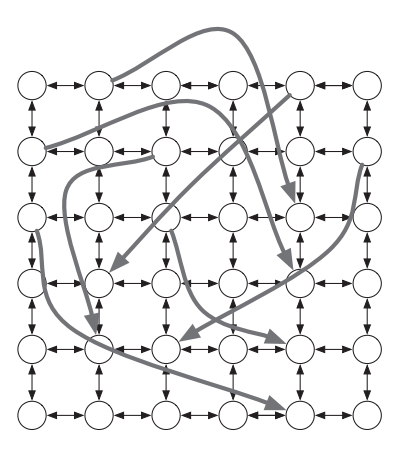
\includegraphics[width=0.5\linewidth]{images/sw_true_network.png}
    \caption{True structure of a network showing the friends of persons. The
    geolocically closer people are the higher the amount of connections. There
    are only few connections over longer range. (source: \cite{networks})}
    \label{fig:oscillation}
\end{figure}


To show that each node can be reached in only six steps, a disease with an infection rate
of 1 and infection duration of 1000 is used. Initially only one
node is infected. Figure %TODO shows the network after x cycles.
After cycle %TODO
all nodes are infected which means they were all able to be reached from the 
starting node in only %TODO
steps.

To reduce the limitation of the used network in regards to the random connections another
network structure could be used. This one closer models the existance of highly coupled
local friend groups where everyone knows each other and a few random connections to people
from other friend groups who are further away. This network uses a high amount of
groups with relatively few members each. In this case 100 groups of 5-10 people are used
and each group of people is connected to 3-4 other groups with only 2-3 edges each.

The same disease is used in this network and the state of the network after cycle %TODO
can be seen in figure %TODO
This shows that in this network it is also possible to reach all other nodes in only six steps,
even though there are only a few long distance connections and a lot of thightly coupled
small groups.


